% !TeX program = lualatex
% !TeX root = luaking.tex
% !TeX encoding = UTF-8
% !TeX spellcheck = cs_CZ
%---------------------------------------------------------------------------------------------------
% file fey1ch45.tex
%---------------------------------------------------------------------------------------------------
%=========================== Kapitola: Ilustrace termodynamiky ====================================
\setchaptertoc
\chapter{Ilustrace termodynamiky}\label{fyz:IchapXLV}
  \section{Vnitřní energie}\label{fyz:IchapXLVsecI}
    Termodynamika je poměrně těžká a složitá ve svých aplikacích a bylo by nepřiměřené, kdybychom se
    v tomto kurzu pouštěli při těchto aplikacích příliš do hloubky. je velmi důležitá pro inženýry a
    chemiky, Zájemci se o ní mohou poučit ve fyzikální chemii nebo inženýrské termodynamice.
    Existuje mnoho dobrých příruček, jako např. Zemanskyho „Teplo a termodynamika“, 
    \begin{itemize}[noitemsep]
      \item Úvod do fyziky v řešených příkladech - (\cite{Havrankova1995}).
      \item Fyzika - Vysokoškolská učebnice obecné fyziky - (\cite{Halliday2001}).
      \item Úvod do fyziky v řešených příkladech - (\cite{Havrankova1995}).
      \item Fundamentals of Thermodynamic - (\cite{Borgnakke2012}).
    \end{itemize}
    v nichž se o termodynamice dozvíme hodně. 

    Termodynamika je tak složitá, protože jednu věc můžeme popsat mnoha způsoby. Chceme-li popsat
    chování plynu, můžeme vycházet z toho, že tlak závisí na teplotě a na objemu nebo z toho, že
    objem závisí na teplotě a tlaku. Zajímáme-li se o vnitřní energii \(U\), můžeme vycházet z toho,
    že závisí na teplotě a objemu, ale proměnné si můžeme zvolit i jinak a pak můžeme vycházet z
    toho, že závisí na teplotě a tlaku nebo na tlaku a objemu apod. V poslední kapitole jsme mluvili
    i jiné funkci teploty a objemu, kterou jsme nazývali entropie a můžeme sestrojit ještě mnoho
    jiných funkcí těchto proměnných: například \(U - TS\) je funkcí teploty a objemu. Máme tedy
    mnoho různých veličin, jež mohou být funkcemi rozmanitých kombinací proměnných. Abychom
    nekomplikovali situaci, budeme v této kapitole uvažovat jako nezávisle proměnné teplotu a objem.
    Chemici používají jako nezávislé proměnné teplotu a tlak, protože se snáze měří a ovládají v
    chemických experimentech, ale my budeme v celé kapitole používat teplotu a objem až na jednu
    výjimku, když budeme vysvětlovat, jak se uskutečňuje transformace na chemický systém proměnných.
    
    Budeme tedy uvažovat jen jeden systém nezávislých proměnných: teplotu a objem. Dalším
    omezením bude to, že se budeme zajímat jen o dvě závislé funkce: o vnitřní energii a tlak. O
    ostatních funkcích nebudeme mluvit, neboť je lze odvodit z uvedených dvou funkcí. I přes tato
    omezení je termodynamika stále dost obtížný předmět, i když už ne tolik.

    \begin{figure}[ht!] %\ref{fyz:fig463}
      \centering
      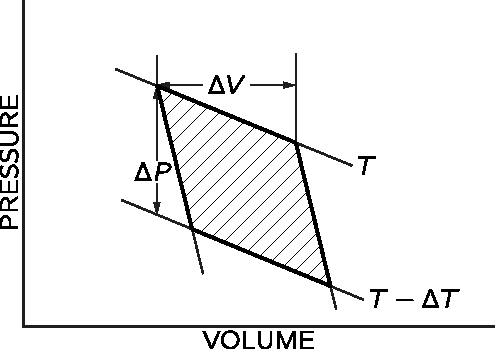
\includegraphics[width=0.7\linewidth]{fyz_fig463.pdf}
      \caption{p-V diagram Carnotova cyklu. Křivky označené \(T\) a \(\Delta T\) jsou izotermy,
               strmější křivky jsou adiabaty. A \(V\) je objemová změna plynu, jemuž bylo při
               konstantní teplotě dodáno teplo \(\Delta\). \(\Delta p\) je změna tlaku plynu, když
               se při konstantním objemu změnila teplota z hodnoty \(T\) na hodnotu \(T - \Delta
               T\). (\cite[s.~615]{Feynman01})}
      \label{fyz:fig463}
    \end{figure}

    \begin{figure}[ht!] %\ref{fyz:fig464}
      \centering
      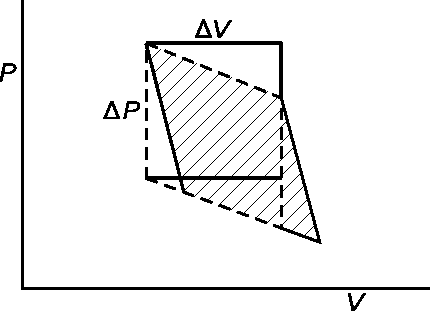
\includegraphics[width=0.7\linewidth]{fyz_fig464.pdf}
      \caption{ 
               (\cite[s.~616]{Feynman01})}
      \label{fyz:fig464}
    \end{figure}

  \section{Aplikace}\label{fyz:IchapXLVsecII}
  \section{Clasiova-Clapeyronova rovnice}\label{fyz:IchapXLVsecIII}
  \section{Příklady a cvičení}\label{fyz:IchapXLVsecIV}
    \subsection{Výhřevnost paliva}\label{fyz:IchapXLVsecIVssecI}
      Výhřevnost \(H\) [\si{\joule\per\kg}] je vlastnost paliva, která udává, kolik energie se
      uvolní úplným spálením jedné jednotky (obvykle \SI{1}{\kg}). Proti spalnému teplu není v
      hodnotě zahrnuto měrné skupenské teplo páry, obsažené ve spalinách. Předpokládá se, že její
      teplo je nevyužitelné a uniká v plynném stavu se spalinami.

      Výhřevnost je dána vztahem
      \begin{equation*}
        H=\dfrac{Q}{m}
      \end{equation*}
      kde \(Q\) je uvolněné teplo a \(m\) je hmotnost paliva. 

      %-Palivo potřebné k letu----------------------------------------
      % !TeX spellcheck = cs_CZ
\begin{mdframed}[style=mdexam]
  \begin{example}\label{FYZ:exam028}
    \emph{Proudové letadlo má čtyři motry, z nich každý vyvíjí tahovu sílu \SI{20}{\kN}. Jaká je
    hmotnost paliva potřebného k letu o délce \SI{5000}{\km}? Výhřevnost paliva je
    \SI{45}{\mega\joule\per\kg}, učinnost motorů \SI{25}{\percent}.(\cite[s.~32]{Bartuska1997})}  

    {\centering
    \captionsetup{type=figure}
    \luafigure[1]{fyz_fig0933.pdf}
    \captionof{figure}{Řez proudovým motorem (\cite[s.~500]{Borgnakke2012})
    \label{fyz:fig0933}}
    \par} 
    
    \textbf{Řešení:}\newline 
    Při práci proudových motorů se část enerige, která se uvolní spálením paliva, spotřebuje na
    vykonání práce. Účinnost motorů je určena vztahem:
    \begin{equation*}
      \eta = \dfrac{W}{Q_1},
    \end{equation*}
    kde \(W = nFs\) je práce, kterou vykonají motory letadla, a \(Q_1 = m_1H\) teplo, které se
    uvolní při letu letadla spálením paliva o hmotnosti \(m_1\) a výhřevnosti \(H\). Užitím těchto
    vztahů dostáváme
    \begin{equation*}
     W = \eta Q_1 = \eta m_1H = nFs \quad\rightarrow\quad m_1 = \dfrac{nFs}{\eta H}.
    \end{equation*}
    Čísleně 
    \begin{align*}
       m_1 &= \dfrac{4\cdot\SI{20}{\kN}\cdot\SI{5000}{\km}}
                    {\num{0.25}\cdot\SI{45}{\mega\joule\per\kg}}                                  \\
       m_1 &= \dfrac{4\cdot\num{2e4}\cdot\num{5e6}}{\num{0.25}\cdot\num{45e6}}\cdot
              \dfrac{\si{\kg\m\per\square\s}\cdot\si{\m}}{\si{\kg\square\m\per\square\s\per\kg}}  \\
       m_1 &\approx \SI{35.6e3}{\kg} \approx \SI{36}{\tonne}        
     \end{align*}
     K letu letadla na dráze \SI{5000}{\km} je zapotřebí palivo o hmotnosti \SI{36}{\tonne}.
  \end{example} 
\end{mdframed}
      %---------------------------------------------------------------
      %-Množství petroleje na ohřátí vody-----------------------------
      % !TeX spellcheck = cs_CZ
\begin{mdframed}[style=mdexam]
  \begin{example}\label{FYZ:exam029}
    \emph{Určete hmotnost petroleje, který spotřebuje petrolejový vařič k zahřátí vody o hmotnosti
    \SI{3}{\kg} z \SI{10}{\degreeCelsius} na \SI{100}{\degreeCelsius}. Účinnost vařiče
    \SI{34}{\percent}, výhřevnost petroleje je \SI{44}{\mega\joule\per\kg} a měrná kapacita vody
    \SI{4180}{\joule\per\kg\per\kelvin}. (\cite[s.~31]{Bartuska1997})}
    
    {\centering
    \captionsetup{type=figure}
    \luafigure[1]{fyz_fig934.png}
    \captionof{figure}{Abychom si v terénu dokázali teplé jídlo připravit, neobejdeme se bez vody a
    bez spolehlivého vařiče a paliva.
    \label{fyz:fig934}}
    \par} 
    
    \textbf{Řešení:}\newline 
    Při ohřívání vody petrolejovým vařičem se jen část tepla, které se uvolní při spalování
    petroleje, spotřebuje na ohřátí vody. Účinnost vařiče je určena vztahem:
    \begin{equation*}
      \eta = \dfrac{Q}{Q_1},
    \end{equation*}
    kde \(Q = mc(t_2 - t_1)\) je teplo, které přijme voda  hmotnosti \(m\) při ohřátí z teploty
    \(t_1\) na teplotu \(t_2\), a \(Q=m_1H\) teplo uvolněné spálením petroleje o hmotnosti \(m_1\)
    a výhřevnosti \(H\). Užitím těchto vztahů dostáváme
    dostáváme
    \begin{align*}
     Q = \eta Q_1 = \eta m_1H &= mc(t_2-t_1) \;\rightarrow  \\
                               m_1 &= \dfrac{mc(t_2-t_1)}{\eta H}.
    \end{align*}
    Čísleně 
    \begin{align*}
       m_1 &= \dfrac{\SI{3}{\kg}\cdot\SI{4180}{\joule\per\kg\per\kelvin}\cdot\SI{90}{\kelvin}}
                    {\num{0.34}\cdot\SI{44}{\mega\joule\per\kg}}                                  \\
       m_1 &= \dfrac{3\cdot4180\cdot90}{\num{0.34}\cdot\num{44e6}}\cdot
              \dfrac{\si{\kg}\cdot\si{\joule\per\kg\per\kelvin}\cdot\si{\kelvin}}
                    {\si{\J\per\kg}}                                                              \\
       m_1 &\approx \SI{75}{\g}    
     \end{align*}
     Na zahřátí vody o hmotnosti \SI{3}{\kg} z \SI{10}{\degreeCelsius} na \SI{100}{\degreeCelsius}
     na petrolejovém vařiči je zapotřebí \SI{75}{\g} petroleje.
  \end{example} 
\end{mdframed}
      %---------------------------------------------------------------
      %-Množství střelného prachu v nábojnici-------------------------
      % !TeX spellcheck = cs_CZ
\begin{mdframed}[style=mdexam]
  \begin{example}\label{FYZ:exam030}
    \emph{Určete hmotnost střelného prachu v nábojnici, jestliže střela má hmotnost \SI{20}{\g} a
    při výstřelu získá rychlost \SI{700}{\m\per\s}. Výhřevnost střelného prachu je
    \SI{3.79}{\mega\joule\per\kg} a účinnost zbraně je \SI{28}{\percent}.
    (\cite[s.~31]{Bartuska1997})}
    
    \textbf{Řešení:}\newline 
    Při výstřelu se část energie, která se uvolní při spálení střelného prachu přemění na kineticku
    energii střely. Účinnost zbraně je určena vztahem:
    \begin{equation*}
      \eta = \dfrac{E_k}{Q_1},
    \end{equation*}
    kde \(E_k = \frac{1}{2}mv^2\) je kinetická energie střeli a \(Q_1 = m_1H\) je celkové teplo,
    které se při výstřelu uvolní spálením střelného prachu o hmotnosti \(m_1\) a výhřevnosti \(H\).
    Užitím těchto vztahů dostáváme dostáváme
    \begin{equation*}
     E_k = \eta Q_1 = \eta m_1H = \frac{1}{2}mv^2 \;\rightarrow\; m_1 = \dfrac{mv^2}{2\eta H}.
    \end{equation*}
    Čísleně 
    \begin{align*}
       m_1 &= \dfrac{\SI{20}{\g}\cdot(\SI{700}{\m\per\s})^2}
                    {2\cdot\num{0.28}\cdot\SI{3.79}{\mega\joule\per\kg}}                          \\
       m_1 &= \dfrac{\num{0.02}\cdot700^2}{\num{0.56}\cdot\num{3.79e6}}\cdot
              \dfrac{\si{\kg}\cdot\si{\square\m\per\square\s}}
                    {\si{\kg\square\m\per\square\s\per\kg}}                                       \\
       m_1 &\approx \SI{4.6}{\g}    
     \end{align*}
     V nábojnici je střelný prach o hmotnosti \SI{4.6}{\g}.
  \end{example} 
\end{mdframed}
      %---------------------------------------------------------------
      %-Automobil-----------------------------------------------------
      % !TeX spellcheck = cs_CZ
\begin{mdframed}[style=mdexam]
  \begin{example}\label{FYZ:exam030}
    \emph{Automobil, jehož motor má výkon \SI{40}{\kW}  a účinnost \SI{28}{\percent}, se pohybuje
    rychlostí \SI{120}{\km\per\hour}. Jakou dráhu může urazit, jestliže zásoba paliva v nádrži je
    \SI{20}{\litre}? Výhřevnost paliva je \SI{46}{\mega\joule\per\kg}, jeho hustota
    \SI{750}{\kg\per\cubic\m}. (\cite[s.~33]{Bartuska1997})}
    
    \textbf{Řešení:}\newline 
    Účinnost automobilového motoru je určena vztahem:
    \begin{equation*}
      \eta = \dfrac{W}{Q_1},
    \end{equation*}
    kde \(W\) je práce, kterou vykoná motor automobilu při jízdě na dráze \(s\) a \(Q_1 = m_1H\)
    teplo, které se při jízdě po této dráze uvolní spálením paliva o hmotnosti \(m_1\) a výhřevnost
    \(H\). Pro práci \(W\) proto platí: 
    \begin{equation*}
     W = \eta Q_1 = \eta m_1H = \eta\varrho VH.
    \end{equation*}
    Výkon automobilového motoru při jízdě na dráze \(s = vt\) je \(P=\dfrac{W}{t}\). Odtud pro práci
    \(W\) dostáváme
    \begin{equation*}
      W = Pt = P\dfrac{s}{t}. 
    \end{equation*}
    Z předchozích rovnic pak vyplývá
    \begin{equation*}
      P\dfrac{s}{t} = \eta\varrho VH \;\rightarrow\; s = \dfrac{\eta\varrho VHv}{P}
    \end{equation*}
    číselně
    \begin{align*}
       s  &=  \dfrac{\num{0.33}\cdot750\cdot\num{30e-3}\cdot\num{46e6}\cdot\num{33.3}}{\num{40e3}}
              \cdot                   
           =  \dfrac{\si{\kg}\cdot\si{\square\m\per\square\s}}
                    {\si{\kg\square\m\per\square\s\per\kg}}                                       \\
       m_1 &\approx \SI{4.6}{\g}    
     \end{align*}
     V nábojnici je střelný prach o hmotnosti \SI{4.6}{\g}.
  \end{example} 
\end{mdframed}
      %---------------------------------------------------------------
    \begin{figure}[ht!] %\ref{fyz:fig465}
      \centering
      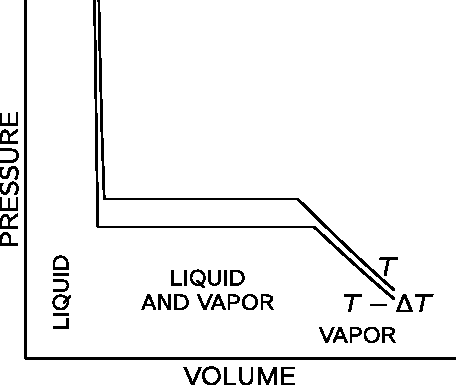
\includegraphics[width=0.7\linewidth]{fyz_fig465.pdf}
      \caption{ 
               (\cite[s.~707]{Feynman01})}
      \label{fyz:fig465}
    \end{figure}

    \begin{figure}[ht!] %\ref{fyz:fig466}
      \centering
      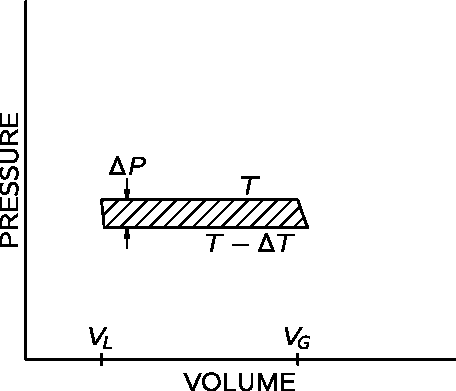
\includegraphics[width=0.7\linewidth]{fyz_fig466.pdf}
      \caption{ 
               (\cite[s.~707]{Feynman01})}
      \label{fyz:fig466}
    \end{figure}
    
    \todo[inline]{Kapitola fey1ch45 je zcela prázdná, pouze obrázky} 
%---------------------------------------------------------------------------------------------------